برای فرمول
$\neg p_3\vee (p_1\to p_3)$
یک دنبالهٔ ساختمان بنویسید و درخت تجزیهٔ آن را رسم کنید.
\begin{ans}
    دنباله ساختمان: 
        $$p_1,p_3,\neg p_3,p_1\to p_3,\neg p_3\vee (p_1\to p_3)$$
    درخت تجزیه:
    \begin{center}
        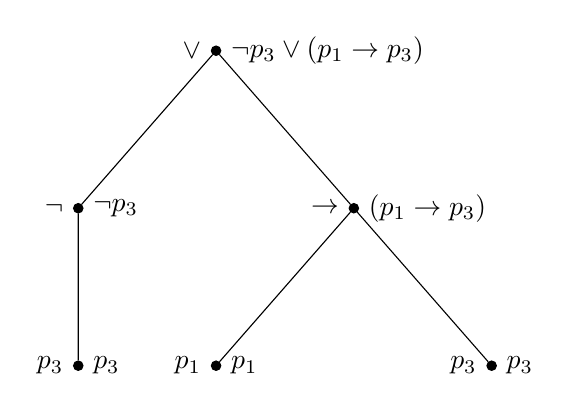
\begin{tikzpicture}
            \tikzset{
                solid node/.style={circle,draw,inner sep=1.2,fill=black},
                hollow node/.style={circle,draw,inner sep=1.2},
                level 1/.style={level distance=20mm,sibling distance=35mm}
            }
            \node {}node[solid node, label = left:$\vee$, label = right:$\neg p_3 \vee (p_1 \to p_3)$]{}
            child { node[solid node, label = left:$\neg$, label = right:$\neg p_3$]{}
                child{ node[solid node, label = left:$p_3$, label = right:$p_3$] {} }
            }
            child { node[solid node, label = left:$\to$, label = right:$(p_1 \to p_3)$] {}
                child { node[solid node, label = left:$p_1$, label = right:$p_1$] {} }
                child { node[solid node, label = left:$p_3$, label = right:$p_3$] {} }
            };
            ]
        \end{tikzpicture}
    \end{center}
\end{ans}
